\section{Database of roll decay tests}
\label{se:database_of_roll_decay_tests}

227 Roll decay tests have been collected with main parameters according to figure \ref{fig:ship_parameters}.

and the parameters in the linear, quadratic and cubic model have been identified using the system identification techniques as described in section \ref{se:system_identification}. The $R^2$ score coefficient was calculated for each model and model test. The mean $R^2$ was 0.995 for the cubic model, 0.993 for the quadratic and 0.986 for the linear model. The quadratic model has almost the same accuracy as the cubic and is therefore chosen to be used for the rest of this project. Figure \ref{fig:roll_decay_model_compare} shows a comparison between the linear, quadratic and cubic model, where it can be seen that the linear model can not give a perfect representation for the whole range of roll angles.    

\begin{figure}[H]
    \centering
    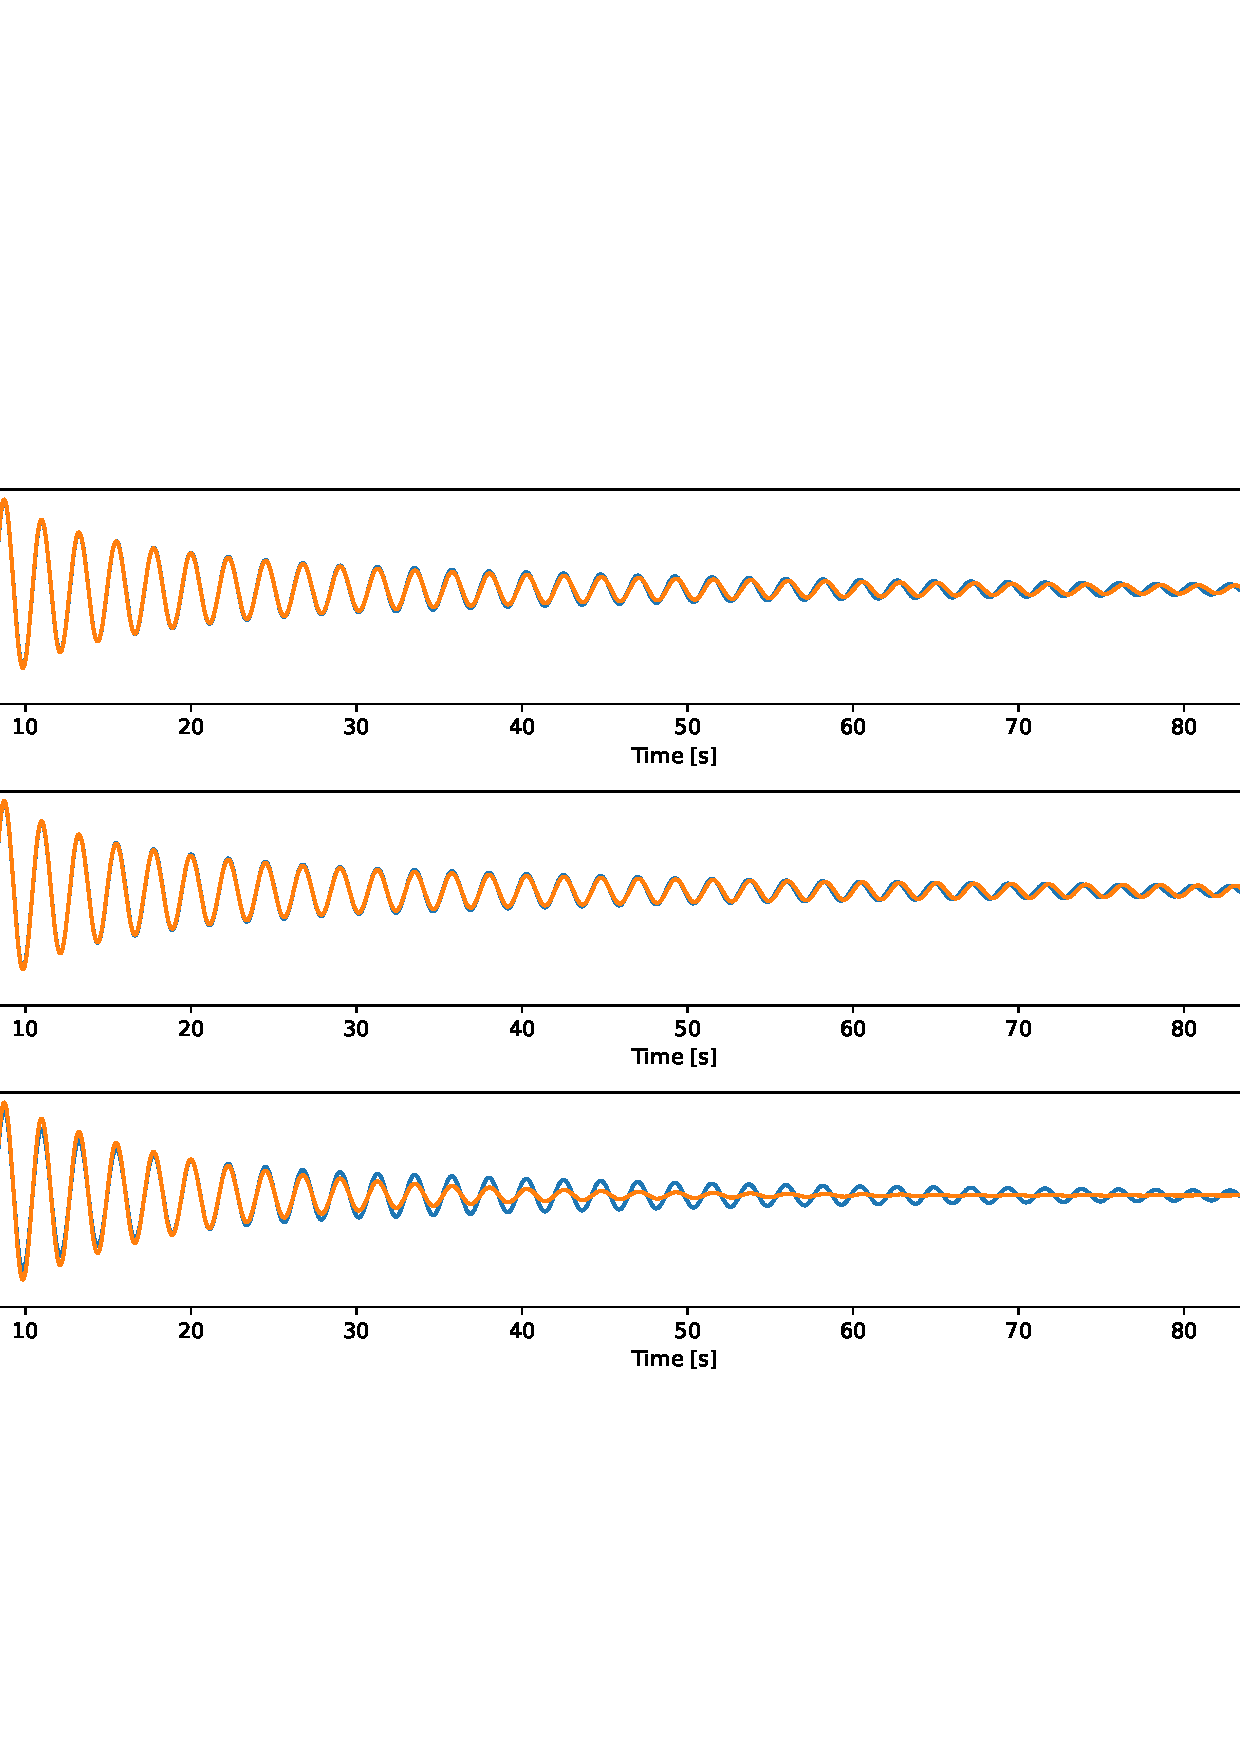
\includegraphics[width=0.9\columnwidth]{figures/roll_decay_model_compare.pdf}
    \caption{Roll decay test comparison of linear, quadratic and cubic model}
    \label{fig:roll_decay_model_compare}
\end{figure}

\begin{figure}[H]
    \centering
    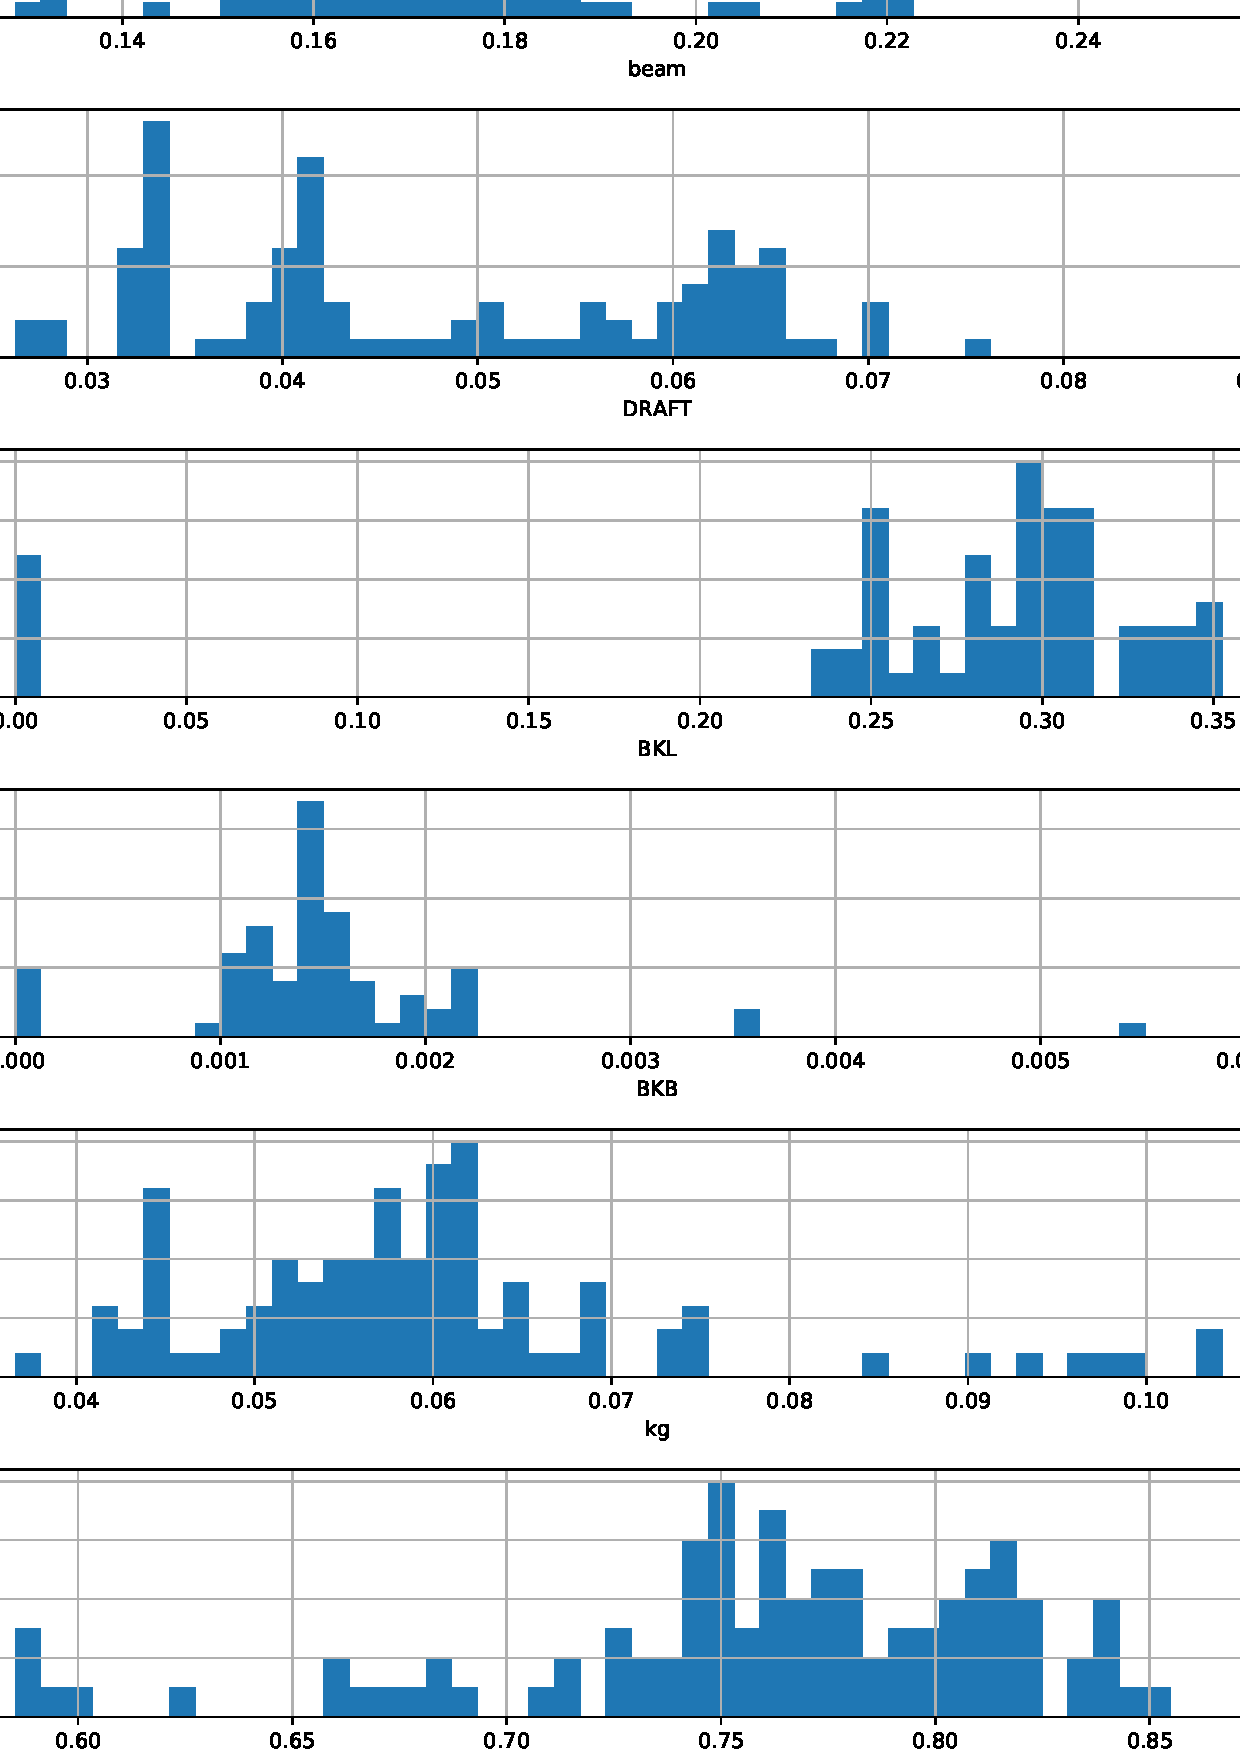
\includegraphics[width=0.9\columnwidth]{figures/ship_parameters.pdf}
    \caption{Histograms of ship parameters from the model tests, all parameters except CB and A0 have been normalized with Lpp}
    \label{fig:ship_parameters}
\end{figure}